\chapter{FX}
\label{FX}
Odin 2 comes with four internal FX modules: \fat{Delay, Chorus, Phaser} and \fat{Flanger}.

\begin{center}
    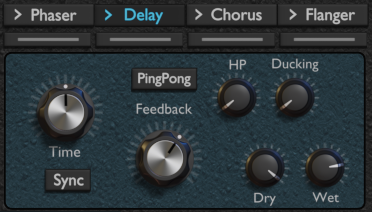
\includegraphics[width=0.4\textwidth]{graphics/FX.png}
\end{center}

The buttons on top of the FX modules serve multiple purposes:

\begin{center}
    
\includegraphics[width=0.4\textwidth]{graphics/FX_selector.png}
\end{center}

Clicking the corresponding name of the module reveals the corresponding module. The buttons below the module name are used to turn enable or disable the module.
You can also \fat{change the order of the modules}, by drag'n'dropping their name handles to the left or right.

\audioparameter{FX On}{0}{1}{
    Use the buttons below the module name to turn the FX module on or off. All modules can be used at the same time.
}

\audioparameter{FX Order}{0}{0}{
    Drag'n'drop the FX module handles to change the order of the FX. The algorithms are calculated in series from left to right.
}

\section{Delay}
\label{delay}
\begin{center}
    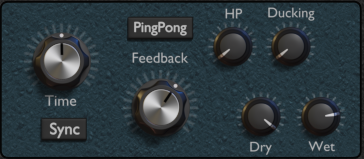
\includegraphics[width=0.5\textwidth]{graphics/delay.png}
\end{center}

A delay is a module capable of producing an 'echo' effect: The signal is fed into a delay-line, which outputs the signal again after a set amount of time again. The output of the delay line can also be fed back in, allowing a chain of attenuating echos. By controlling the delay time and feeback parameters, a wide variety of effects can be achieved. The Delay module in Odin 2 goes a step further and offers several additional features.

\audioparameter{Delay Time}{1}{1}{
    Controls the time the delay line takes to output the sound again. Depending on the parameter "Delay Sync", this is either a dial for continuous values in Hz, or a custom selector to sync the time to the beat. This selector allows for arbitrary fractions of the current host BPM, for example 5/16th notes:

    \begin{center}
        
\includegraphics[width=0.18\textwidth]{graphics/delay_sync.png}
    \end{center}
}

\audioparameter{Delay Feedback}{1}{1}{
    Controls how much of the output of the delay line is fed back in again. If feedback is zero, only one echo will be audible. If feedback is one, an infinite series of exact copies of sound will be output. Everything inbetween makes for slowly attenuating echos.
}

\audioparameter{Delay Sync}{0}{1}{
    Controls whether the Delay Time is set by a knob in Hz or via the sync-time selector, syncing it to the host BPM.
}

\audioparameter{Delay PingPong}{0}{1}{
    Enabling PingPong will make the left and right stereo delay lines crossfeed: The output of the left line is fed into the right line and vice versa.

    The initial input into the delay lines is mixed down to a mono signal and then fed into the left delay line only. The dry signal remains in the center of the stereo field.
}

\audioparameter{Delay Highpass (HP)}{1}{1}{
    The processed signal in the Delay module is filtered through a 6dB/Oct highpass filter. The Delay Highpass parameter controls the cutoff of this internal filter. This is great for removing the muddiness that deep frequencies can produce in a delay module.

    Note that the highpass filter is not applied inside, but after the feedback loop, i.e. consecutive echos do not get filtered further more as they are processed again.
}

\audioparameter{Ducking}{0}{1}{
    Ducking attenuates the output of the delayed signal if an input signal is present. This is great for decluttering sections where the delayed signal interferes with the unprocessed signal.
}

Unlike the other FX modules, the Delay features a separate Dry and Wet control to allow for easier adjustments of processed and unprocessed signals individually.
\audioparameter{Delay Dry}{1}{1}{
    Controls how much unprocessed signal is output by the Delay.
}

\audioparameter{Delay Wet}{1}{1}{
    Controls how much processed signal is output by the Delay.
}

\section{Chorus}
\begin{center}
    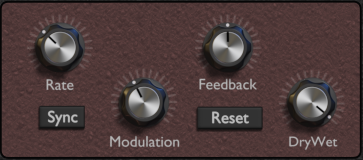
\includegraphics[width=0.5\textwidth]{graphics/chorus.png}
\end{center}

The Chorus module is a delay based effect capable of thickening sounds. The generated sound resembles that of a slightly detuned ensemble, hence the name chorus. Internally, the Chorus module uses a delay line, which is read from at two diferent positions. The delay times are modulated by an internal Low Frequency Oscillator (LFO). This slightly detunes the result resulting in the Chorus sound. The LFOs for the left and right channel are phase-offset by 90° to spread the sound in the stereo field.

\audioparameter{Chorus Rate}{1}{1}{
    Controls the speed of the internal LFO. Depending on the parameter "Chorus Sync", this is either a dial for continuous values in Hz, or a custom selector to sync the time to the beat. This selector allows for arbitrary fractions of the current host BPM, for example 5/16th notes:

    \begin{center}
        
\includegraphics[width=0.18\textwidth]{graphics/chorus_sync.png}
    \end{center}
}

\audioparameter{Chorus Sync}{0}{1}{
    Controls whether the Chorus Rate is set by a knob in Hz or via the sync-time selector, syncing it to the host BPM.
}

\audioparameter{Chorus Modulation}{1}{1}{
    Controls how much the internal LFO modulates the two delay times. Exaggerates the detune effect.
}

\audioparameter{Chorus Feedback}{1}{1}{
    Controls how much of the output of the delay line is fed back in again. Pronounces the effect of the Chorus a bit more.
}

\audioparameter{Chorus DryWet}{1}{1}{
    Interpolates the processed and unprocessed signals, thereby controlling the strength of the effect.
}

\section{Phaser}
\begin{center}
    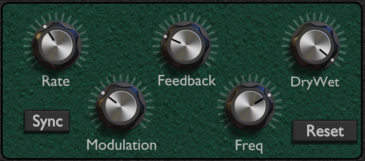
\includegraphics[width=0.5\textwidth]{graphics/phaser.png}
\end{center}
The phaser module introduces movement to the sound by applying a subtle "windy" character. The internal structure consists of a series of allpass filters: These filters do not alter the amplitude like the filters from Chapter \ref{filters}, but only shifts the phase of some frequencies. By adding the phase-shifted signal back onto the original signal, some of the frequencies get boosted, attenuated or eliminated entirely via phase-cancellation. The characteristic of the allpass-filters is continuously modulated by an internal Low Frequency Oscillator (LFO), which makes for the movemnet in the sound. The LFOs for the left and right channel are phase-offset by 90° to spread the sound in the stereo field.

\audioparameter{Phaser Rate}{1}{1}{
    Controls the speed of the internal LFO. Depending on the parameter "Phaser Sync", this is either a dial for continuous values in Hz, or a custom selector to sync the time to the beat. This selector allows for arbitrary fractions of the current host BPM, for example 5/16th notes:

    \begin{center}
        
\includegraphics[width=0.18\textwidth]{graphics/phaser_sync.png}
    \end{center}
}

\audioparameter{Phaser Sync}{0}{1}{
    Controls whether the Phaser Rate is set by a knob in Hz or via the sync-time selector, syncing it to the host BPM.
}

\audioparameter{Phaser Modulation}{1}{1}{
    Controls how much the internal LFO modulates the internal allpass filters.
}

\audioparameter{Phaser Feedback}{1}{1}{
    An extra feedback stage, which feeds the output signal into the input again.
}

\audioparameter{Phaser Freq}{1}{1}{
    Shifts the base frequency of the internal allpass filters, thereby altering the characteristic of the effect.
}

\audioparameter{Phaser DryWet}{1}{1}{
    Controls how much of the phase-shifted signal is added to the input signal, thereby controling the strength of the effect.
}

\section{Flanger}
\begin{center}
    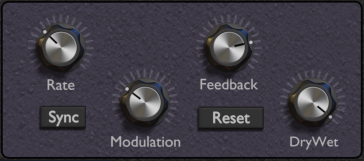
\includegraphics[width=0.5\textwidth]{graphics/flanger.png}
\end{center}

A Flanger is a modulated \hyperref[comb_filter]{comb filter}. The signal is fed into a delay line and mixed with the input signal after a small echo. The timing of this effect is modulated by an internal Low Frequency Oscillator (LFO). Additionally, the output of the delay line can be fed in again via the Feedback parameter, to allow for a continuous stream of echoes. The delay times for Comb Filters and Flangers is very short, usually below 50ms. 

\audioparameter{Flanger Rate}{1}{1}{
    Controls the speed of the internal LFO. Depending on the parameter "Flanger Sync", this is either a dial for continuous values in Hz, or a custom selector to sync the time to the beat. This selector allows for arbitrary fractions of the current host BPM, for example 5/16th notes:

    \begin{center}
        
\includegraphics[width=0.18\textwidth]{graphics/flanger_sync.png}
    \end{center}
}

\audioparameter{Flanger Sync}{0}{1}{
    Controls whether the Flanger Rate is set by a knob in Hz or via the sync-time selector, syncing it to the host BPM.
}

\audioparameter{Flanger Modulation}{1}{1}{
    Controls how much the internal LFO modulates the delay time.
}

\audioparameter{Flanger Feedback}{1}{1}{
    Controls how much of the output of the delay line is fed back in again. Creates a metallic smearing effect for big values. This parameter can be positive or negative allowing for positive and negative comb operation.
}

\audioparameter{Flanger DryWet}{1}{1}{
    Interpolates the processed and unprocessed signals, thereby controlling the strength of the effect.
}